\section{Results}

\subsection{Evidence Ladder}

The paper advances through a deliberate evidence ladder: fully real symbol-level evidence from the frozen workshop package, synthetic-from-real grouped and downstream evidence from the stronger sequence branch, replicated real grouped evidence on two corpora, and a redesigned real downstream task with improved coverage. Table~\ref{tab:bridge} keeps that claim boundary explicit without trying to narrate the whole paper in one artifact. The Historical Newspapers trust hardening sits behind this ladder rather than inside it, and Appendix Table~\ref{tab:appendix_trust} records that audit chain directly.

\begin{table*}[t]
\caption{Evidence ladder for the paper's main claims.}
\label{tab:bridge}
\centering
\footnotesize
\setlength{\tabcolsep}{4pt}
\renewcommand{\arraystretch}{1.08}
\begin{tabular}{|p{1.8cm}|p{3.0cm}|p{2.6cm}|p{7.0cm}|}
\hline
\textbf{Tier} & \textbf{Data and task} & \textbf{Main signal} & \textbf{Boundary it supports} \\
\hline
Real symbol level & Frozen workshop symbol benchmark & Top-k delta $+$0.224 & Fully real symbol-level uncertainty retention remains the strongest clean real result. \\
\hline
Synthetic grouped & Omniglot, Digits, Kuzushiji-49 Markov sequences & Exact delta $+$0.019, top-k delta $+$0.073 & Higher-level grouped gains exist beyond symbol level, but the structure is synthetic-from-real. \\
\hline
Synthetic downstream & Process-family recovery & Family delta $+$0.048 & Downstream structural gains exist on synthetic-from-real tasks, but they are selective. \\
\hline
Real grouped replication & Historical Newspapers and ScaDS.AI grouped words & Top-k delta $+$0.181, CI [$+$0.122, $+$0.236] & Grouped top-k rescue replicates across two real grouped token-aligned corpora. \\
\hline
Real grouped exact & Same two real corpora & Conformal exact delta $+$0.059 & Exact grouped recovery remains mixed rather than cleanly replicated. \\
\hline
Real downstream redesign & Two real grouped corpora, train-supported n-gram path & Coverage upper bound 0.833; raw exact delta $-$0.028; conformal exact delta $+$0.059 & The downstream task is no longer coverage-starved, but exact real downstream gains remain selective. \\
\hline
Real-data trust & Historical Newspapers audit and gold-style pass & 2/126 token changes; zero metric drift & The Historical Newspapers grouped result is strong enough for a bounded real grouped-recognition claim. \\
\hline
\end{tabular}
\end{table*}


\subsection{Replicated Real Grouped Transfer}

The cleanest new real result is grouped top-k replication across Historical Newspapers and ScaDS.AI. Historical Newspapers shows a mean grouped top-k delta of +0.056, ScaDS.AI shows +0.306, and the two-corpus mean grouped top-k delta is +0.181. Example-level bootstrap analysis gives a confidence interval of [+0.122, +0.236] with bootstrap probability 1.000 for a positive mean effect. Figure~\ref{fig:storyline} makes the paper's core contrast visible in one place: the real grouped signal replicates, but downstream propagation is gated by support regime rather than arriving automatically.

\begin{figure*}[!t]
\centering
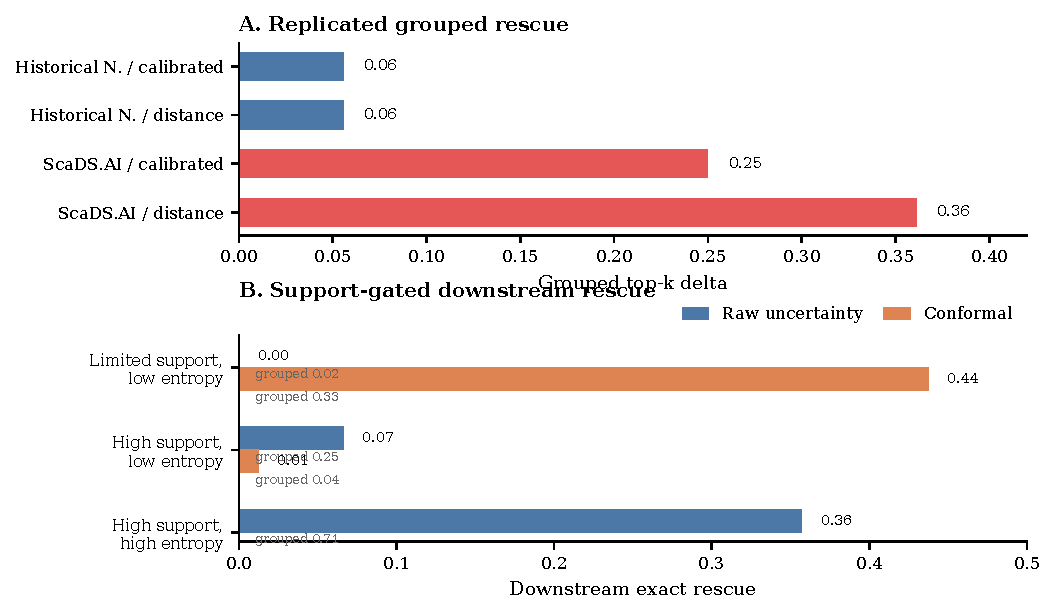
\includegraphics[width=0.98\textwidth]{figures/fig1_propagation_regime_plot}
\caption{From replicated grouped rescue to support-gated downstream rescue. Panel A shows the paper's strongest replicated real-data signal: grouped top-k rescue is positive on both real grouped corpora across both posterior families. Panels B and C show the explanatory result: downstream rescue depends on support regime, and raw uncertainty versus conformal help in different parts of that space.}
\label{fig:storyline}
\end{figure*}

\subsection{Redesigned Real Downstream Task}

The redesigned downstream task removes much of the previous coverage collapse, but it does not convert the branch into a clean replicated exact downstream paper. Selective positive cases do appear. ScaDS.AI with cluster-distance posteriors shows a raw exact downstream delta of +0.111, and Historical Newspapers under cluster-distance posteriors shows a conformal exact downstream delta of +0.222 over raw uncertainty. Across both real corpora, however, the mean raw exact downstream delta remains -0.028 and the mean conformal exact downstream delta is +0.059. The raw interval crosses zero, while the conformal interval remains positive. Appendix Figure~\ref{fig:appendix_downstream} and Table~\ref{tab:appendix_robustness} keep the coverage and bootstrap details visible without crowding the main narrative.

\subsection{Propagation Analysis}

The propagation analysis is the main analytical contribution. Symbol rescue is the clearest grouped-rescue predictor, with odds ratio about 18.4. On the real downstream task, grouped top-k delta is the strongest positive downstream predictor, with odds ratio about 6.1. Grouped rescue is therefore necessary but not sufficient for downstream success.

The rate summaries reinforce that interpretation. Grouped-rescue rate rises by about 0.085 when symbol rescue is present, with bootstrap interval [0.072, 0.099]. Downstream exact-rescue rate rises by about 0.375 when grouped rescue is present, with bootstrap interval [0.275, 0.475]. The most stable downstream threshold is grouped top-k delta greater than or equal to one recovered alternative, while entropy thresholds are informative but less stable across posterior families.

Figure~\ref{fig:storyline} shows that raw uncertainty and conformal help in different parts of the support space. Raw uncertainty helps most in rare high-support, high-entropy regions, whereas conformal helps more in limited-support, low-entropy regions. The explanation is therefore regime-aware rather than monotonic: local rescue can be real and replicated, but its downstream usefulness still depends on measurable support conditions.
